\documentclass[remotesensing,article,submit,moreauthors,pdftex,10pt,a4paper]{Definitions/mdpi} 

    \firstpage{1} 
    \makeatletter 
    \setcounter{page}{\@firstpage} 
    \makeatother
    \pubvolume{xx}
    \issuenum{1}
    \articlenumber{5}
    \pubyear{2018}
    \copyrightyear{2018}
    %\externaleditor{Academic Editor: name}
    \history{Received: date; Accepted: date; Published: date}

    \usepackage{gensymb}
    \usepackage{cleveref}
    \usepackage{xcolor}
    \Title{%
    Complementarity Between Sentinel-1 and Landsat 8 Imagery
    for Built-Up Mapping in Sub-Saharan Africa}

    \newcommand{\orcidauthorA}{0000-0001-7275-7967}
    \newcommand{\orcidauthorB}{0000-0001-5487-6137}
    \newcommand{\orcidauthorC}{0000-0003-3708-3359}
    \newcommand{\orcidauthorD}{0000-0002-0819-7755}

    \Author{%
    Yann Forget $^{1}$\orcidA{}*,
    Michal Shimoni $^{2}$\orcidB{},
    Marius Gilbert $^{1}$\orcidC{} and
    Catherine Linard $^{3}$\orcidD{}}

    \AuthorNames{Yann Forget, Michal Shimoni, Marius Gilbert and Catherine Linard}

    \address{%
    $^{1}$ \quad Spatial Epidemiology Lab (SpELL), Université Libre de Bruxelles, Brussels, Belgium.\\
    $^{2}$ \quad Signal and Image Centre, Belgian Royal Military Academy (SIC-RMA), Brussels, Belgium.\\
    $^{3}$ \quad Department of Geography, University of Namur, Namur, Belgium.}

    \corres{Correspondence: yannforget@mailbox.org}

    \abstract{%
    The rapid urbanization that takes place in developing regions such as
    Sub-Saharan Africa is associated with a large range of environmental and
    social issues. In this context, remote sensing is essential to provide
    accurate and up-to-date spatial information to support risk assessment and
    decision making. However, mapping urban areas remains a challenge because of
    their heterogeneity, especially in developing regions where the highest
    rates of misclassification are observed. Nevertheless, urban areas located
    in arid climates --- which are among the most vulnerables to anthropogenic
    impacts, suffer from the spectral confusion occurring between built-up and
    bare soil areas when using optical imagery. Today, the increasing
    availability of satellite imagery from multiple sensors allow to tackle the
    aforementioned issues by combining optical data with Synthetic Aperture
    Radar (SAR). In this paper, we assess the complementarity of the Landsat 8
    and Sentinel-1 sensors to map built-up areas in twelve Sub-Saharan African
    urban areas, using a pixel-level supervised classification based on the
    Random Forest classifier. We make use of textural information extracted from
    SAR backscattering data in order to reduce the speckle noise and to
    introduce contextual information at the pixel level. Results suggest that
    combining both optical and SAR features consistently improves classification
    performances, mainly by enhancing the differentiation between built-up and
    bare lands. However, the fusion was less beneficial in mountainous case
    studies, suggesting that including features derived from a Digital Elevation
    Model (DEM) could improve the reliability of the proposed approach. As
    suggested by previous studies, combining features computed from both VV and
    VH polarizations consistently led to better classification performances. On
    the contrary, introducing textures computed from different spatial scales
    did not improve the classification performances.}

    \keyword{%
    Urban Remote Sensing; Sentinel-1; Landsat 8; Built-Up; Data Fusion; Texture; Africa}

\begin{document}

\section{Introduction}

Urbanization is a worldwide process associated with a wide range of
environmental and human health issues \cite{Grimm2008, Dye2008}. In Africa, the
urban population is predicted to triple between 2010 and 2050, threatening both
social and environmental sustainability \cite{UN-Habitat2015}. Monitoring
built-up areas in developing regions such as Sub-Saharan Africa is therefore
crucial to understand, predict, and mitigate the risks associated with such a
rapid urbanization \cite{Linard2013}. In this context, remote sensing plays a
major role by providing accurate spatial information on built-up areas at a
relatively low cost \cite{Gamba2009, Wentz2014}. However, because of the
heterogeneity of urban areas in terms of spatial structure and materials,
mapping built-up with medium resolution optical imagery remains challenging. In
medium spatial resolution imagery (10-50 meters), urban pixels are made of a
combination of several elements --- such as buildings, roads, trees or bare
soil. Furthermore, the spectral characteristics and the spatial distribution of
these objects differ across a given urban area. High differences are also
observed among the cities of the world because of socioeconomic, cultural,
historical and environmental variations \cite{Forster1993, Small2001,
Small2005}. Developing regions are the most concerned with the
urbanization-related risks, --- but previous studies have shown that they also
suffer from lower accuracies in global built-up maps \cite{Potere2009}, because
of a high urban heterogeneity coupled with a lack of reference datasets to
support the training and the validation of the classification models.

Likewise, urban areas located in arid and semi-arid climates are among the most
vulnerables to anthropogenic impacts. Despite the fact that about one third of
the global land surface is characterized by an arid or semi-arid climate
according to the Köppen-Geiger classification \cite{Kottek2006, Rubel2017}, they
also suffer from low accuracies when it comes to built-up mapping. Due to their
overlapping spectral signatures, the differentiation between bare land and
built-up in arid and semi-arid environments has proven to be one of the main
challenge associated with optical sensors in urban remote sensing. Previous
studies have shown that conventional spectral indices --- such as the normalized
difference built-up index (NDBI), the normalized difference bareness index
(NDBal), or the urban index (UI), are not reliable to differentiate built-up
areas from bare land in arid regions \cite{Qian2007, Rasul2018}. As a result,
new approaches based on object-oriented classification or linear spectral
mixture analysis have been proposed \cite{Qian2007, Zhang2015}. New spectral
indices have also been specifically developed to tackle the issue, such as the
normalized bare land index (NBLI) \cite{Li2017}. Likewise, the dry built-up
index (DBI) and the dry bare-soil index (DBSI) provide a better separation
between bare soil and built-up in arid regions by making use of the blue and
thermal bands of Landsat 8 \cite{Rasul2018}. Approaches based on the
thresholding of spectral indices do not require any training dataset and benefit
from a low computational cost. However, as stated by their authors, their
reliability highly depends on the landscape and the climate of the study area.
For instance, the DBSI is not considered suitable in humid regions or in urban
areas surrounded by vegetation \cite{Rasul2018}.

Because of the aforementioned issues, the idea of combining optical data with
complementary sensors such as Synthetic Aperture Radar (SAR) recently gained
momentum. SAR has the advantages of providing high resolution imagery
independently from daylight, clouds, or weather conditions. The C-band of the
European Remote-Sensing Satellite 1 and 2 (ERS-1/2) has been widely used to
monitor urban areas \cite{Weng2014a}. However, in contrast to optical sensors,
SAR is sensitive to the roughness of the terrain --- and thus is able to better
differentiate between bare soil and built-up \cite{Soergel2010}. Previous
studies have shown that the combined use of optical and SAR data can
significantly improves the accuracy of a land cover classification
\cite{Waske2008, Zhang2012, Joshi2016}. However, classifying data provided by
different sensors is not straightforward and there is no consensus among the
remote sensing community regarding the best fusion approach. Conventional
parametric classifiers which concatenate signals from different sensors into one
vector have been shown to be inefficient in modeling multi-sensor data
distributions, therefore most of the methods rely on machine learning
classifiers that do not make any assumption regarding the data distribution
\cite{Tupin2010}. Fusion can occur at four different levels: (1) at the signal
level, (2) at the pixel level --- by concatenating data from multiple sensors
into one stacked vector \cite{Griffiths2010, Zhu2012a, Zhang2014b, Braun2015},
(3) at the feature level in the context of an object-based classification that
makes use of image segmentation techniques \cite{Clerici2017}, or (4) at the
decision level, for instance by merging several single-source classifiers using
neural networks or support vector machines \cite{Benediktsson1999, Fauvel2006,
Waske2008, Shao2016}.

Previous studies have reported that pixel-level fusion approaches are
inappropriate because of the lack of information about the spatial context of a
given pixel and the speckle noise inherent to SAR data \cite{Tupin2010,
Gamba2014, Zhang2014b}. The extraction of textural features from SAR
backscattering partially solves the aforementioned issues \cite{Zhang2014b,
Braun2015}, for instance by computing the grey level co-occurrence matrix (GLCM)
texture features \cite{Haralick1973, Gotlieb1990}. However, there is no
consensus on which features are the most relevant in the context of a combined
use with optical data, or on the optimal size of the moving window used to
compute the GLCM.

In this paper, we investigate the combined use of Landsat 8 and Sentinel-1
imagery to detect built-up in twelve Sub-Saharan African case studies
characterized by various climates, landscapes and population patterns. We assess
the complementarity of optical and SAR data in the context of a pixel-level
supervised classification based on the extraction of 18 GLCM texture features,
with several window sizes and from the two polarizations available with
Sentinel-1 --- VV and VH.

\section{Materials and methods}

\subsection{Case studies}

\begin{table}[H]
	\caption{%
		Climate, topography and population for each case study. Values are
		aggregated for the area of interest. Climate data is derived from the
		Koppen-Geiger classification \cite{Kottek2006, Rubel2017}. Mean slope and
		elevation are computed from the Shuttle Radar Topographic Mission (SRTM) 30m
		\cite{NASAJPL2013}. Population is estimated using the AfriPop/WorldPop
		dataset \cite{Linard2012b, Worldpop2016}}
	\centering
	\begin{tabular}{llrrr}
		\toprule
		\textbf{City (Country)} & \textbf{Climate}     & \textbf{Mean slope} & \textbf{Mean elevation} & \textbf{Population} \\
		\midrule
		Antananarivo (MDG)      & Subtropical highland & 8\degree            & 1319 m                  & 2,436,196           \\
		Bukavu (COD)            & Subtropical highland & 13\degree           & 1836 m                  & 1,041,703           \\
		Chimoio (MOZ)           & Humid subtropical    & 4\degree            & 612 m                   & 455,612             \\
		Dakar (SEN)             & Hot semi-arid        & 2\degree            & 14 m                    & 3,332,985           \\
		Gao (MLI)               & Hot desert           & 3\degree            & 273 m                   & 161,172             \\
		Johannesburg (ZAF)      & Subtropical highland & 4\degree            & 1608 m                  & 4,668,844           \\
		Kampala (UGA)           & Tropical rainforest  & 5\degree            & 1177 m                  & 3,498,376           \\
		Katsina (NGA)           & Hot semi-arid        & 2\degree            & 495 m                   & 1,027,729           \\
		Nairobi (KEN)           & Temperate oceanic    & 4\degree            & 1692 m                  & 5,064,548           \\
		Ouagadougou (BFA)       & Hot semi-arid        & 2\degree            & 308 m                   & 2,256,479           \\
		Saint-Louis (SEN)       & Hot desert           & 2\degree            & 7 m                     & 300,518             \\
		Windhoek (NAM)          & Hot desert           & 9\degree            & 1811 m                  & 383,503             \\
		\bottomrule
	\end{tabular}
	\label{tbl:case-studies}
\end{table}

Compared to natural land covers, built-up areas are highly heterogeneous at both
the interurban and the intraurban scales. As a result, a method developed in the
context of an european urban areas has no guarantee to be reliable in a small
urban agglomeration of Sub-Saharan Africa. This is why a diverse set of case
studies is crucial when seeking to maximize the generalization potential of a
method. In the context of built-up mapping using both optical and SAR data, the
reliability of each sensor is expected to be highly dependent on landscape and
climate variables. The selected case studies for the present analysis are
presented in \autoref{tbl:case-studies}. The area of interest for each case
study corresponds to the rectangular 20 kilometers buffer around the city
center.

The set contains urban areas with various climates, landscapes and population
characteristics. In the context of built-up mapping from both optical and SAR
data, optical sensors are expected to perform well in tropical, subtropical and
temperate climates (Antananarivo, Bukavu, Chimoio, Kampala or Johannesburg)
because of their ability to differentiate between the spectral signatures of
built-up and vegetation. However, densely vegetated urbain mosaics could cause
some confusion. On the contrary, SAR sensor is expected to perform better in dry
climates (Dakar, Gao, Katsina, Saint-Louis, Ouagadougou or Windhoek), and lower
in mountainous urban areas surrounded with dense vegetation and steep slopes
(Antananarivo, Bukavu, or Windhoek). More generally, the various climates and
population sizes ensure that multiple urban morphologies will be encountered.

\subsection{Data Acquisition and Preprocessing}

\begin{table}[H]
	\caption{Sentinel-1 and Landsat 8 product types and acquisition dates.}
	\centering
	\label{tbl:satellite-imagery}
	\begin{tabular}{lcc}
		\toprule
		             & \textbf{Sentinel-1}                & \textbf{Landsat 8} \\
		\midrule
		Antananarivo & \texttt{S1A\_IW\_GRDH\ 2015-10-07} &                    
		\texttt{LC08\_L1TP\ 2015-06-15}\tabularnewline
		Bukavu       & \texttt{S1A\_IW\_GRDH\ 2016-06-10} &                    
		\texttt{LC08\_L1TP\ 2015-09-21}\tabularnewline
		Chimoio      & \texttt{S1A\_IW\_GRDH\ 2015-04-27} &                    
		\texttt{LC08\_L1TP\ 2016-03-28}\tabularnewline
		Dakar        & \texttt{S1A\_IW\_GRDH\ 2016-05-12} &                    
		\texttt{LC08\_L1TP\ 2015-12-17}\tabularnewline
		Gao          & \texttt{S1A\_IW\_GRDH\ 2016-06-13} &                    
		\texttt{LC08\_L1TP\ 2016-07-08}\tabularnewline
		Johannesburg & \texttt{S1A\_IW\_GRDH\ 2015-10-20} &                    
		\texttt{LC08\_L1TP\ 2015-12-21}\tabularnewline
		Kampala      & \texttt{S1A\_IW\_GRDH\ 2016-07-04} &                    
		\texttt{LC08\_L1TP\ 2016-01-29}\tabularnewline
		Katsina      & \texttt{S1A\_IW\_GRDH\ 2016-05-12} &                    
		\texttt{LC08\_L1TP\ 2015-10-23}\tabularnewline
		Nairobi      & \texttt{S1A\_IW\_GRDH\ 2016-10-27} &                    
		\texttt{LC08\_L1TP\ 2016-01-24}\tabularnewline
		Ouagadougou  & \texttt{S1A\_IW\_GRDH\ 2015-04-13} &                    
		\texttt{LC08\_L1TP\ 2016-12-22}\tabularnewline
		Saint-Louis  & \texttt{S1A\_IW\_GRDH\ 2016-06-05} &                    
		\texttt{LC08\_L1TP\ 2016-10-09}\tabularnewline
		Windhoek     & \texttt{S1B\_IW\_GRDH\ 2016-10-09} &                    
		\texttt{LC08\_L1TP\ 2016-01-14}\tabularnewline
		\bottomrule
	\end{tabular}
\end{table}

Sentinel-1 and Landsat 8 product types and acquisition dates are presented in
\autoref{tbl:satellite-imagery}. Landsat 8 imagery was acquired through the
Earth Explorer portal of the U.S. Geological Survey (USGS) with the
\texttt{landsatxplore} software \cite{Forget2018}, using cloud cover as the main
criterion. Additionally, monthly NDVI values from the MODIS-based MOD13C2
dataset \cite{Didan2015} were used to favor the most vegetated periods, which
are different depending on the case study. Scenes were acquired as Level-1 data
products, thus radiometrically calibrated and orthorectified. Calibrated digital
numbers were converted to surface reflectance values using the Landsat Surface
Reflectance Code (LaSRC) \cite{Vermote2016} made available by the USGS. Cloudy
pixels were masked using the Function of Mask (FMASK) algorithm \cite{Zhu2012,
Zhu2015}.

Sentinel-1A images were acquired through the Copernicus Open Access
Hub using the \texttt{sentinelsat} software \cite{Clauss2018}. Scenes belonging
to the dry season were favored based on the monthly NDVI values provided by the
MODIS-based MOD13C2 dataset. Additionally, the CPC Global Unified Precipitation
dataset \cite{Chen2008}, provided by the NOAA Climate Prediction Center, was
used to require at least two days without any precipitation before the
acquisition date. The last criterion for the final scene selection was the
temporal proximity to the selected Landsat 8 scene. The scenes were acquired as
Ground Range Detected (GRD) Level-1 products in the Interferometric Wide (IW)
swath mode, therefore multi-looked and projected to ground range using an Earth
ellipsoid model. Preprocessing was performed using the Sentinel Application
Platform (SNAP) \cite{ESA2018}. Firstly, orbit state vectors were refined with
precise orbit files and GRD data was calibrated to \(\beta\) nought. Then,
thermal noise removal was performed before applying a speckle noise reduction
based on a \(3 \times 3\) Lee filter \cite{Lee1981}, in order to reduce the
speckle noise while preserving the textural information. Finally, terrain
flattening \cite{Small2011} and Range-Doppler terrain correction
\cite{Small2008} were applied based on the SRTM 1-sec Digital Elevation Model
(DEM).

\subsection{Feature Extraction}

Grey Level Co-Occurence Matrix (GLCM) textures were computed with an interpixel
distance of 1 and 32 levels of quantization using Orfeo Toolbox
\cite{Grizonnet2017}, after a \(2\%\) histogram cutting on the source SAR data.
GLCMs were constructed for the direction angles 0, 45, 90, and 135 degrees ; but
only the average value was considered. The GLCMs were computed independently for
each polarization (VV and VH) and multiple window sizes (\(5 \times 5\), \(7
\times 7\), \(9 \times 9\), and \(11 \times 11\)). A set of 18 textures was
extracted: energy, entropy, correlation, inertia, cluster shade, cluster
prominence, haralick correlation, mean, variance, dissimilarity, sum average,
sum variance, sum entropy, difference of entropies, difference of variances, and
two information measures of correlation (IC1 and IC2). This resulted in the
extraction of 72 texture features for each polarization, that is, 144 in total.

Several GLCMs texture features can be highly correlated, such as energy and
entropy, or inertia and the inverse different moment. In order to reduce the
dimensionality of the dataset, a Principal Component Analysis (PCA) was
performed on each combination of polarization and window size. Only the first
six components of each PCA --- which consistently explained more than 95\% of
the variance, were retained. This reduced the number of features from 144 to 48.

SAR features were reprojected to Universal Transverse Mercator (UTM) coordinate
system only after the computation of GLCM textures in order to minimize the
destruction of textural information. All Landsat 8 bands --- including thermal
bands, were retained without further processing except of co-registration to the
spatial resolution of SAR products (i.e.~about 10 meters).

\subsection{Classification}

The binary classification task --- built-up vs.~non-built-up, was
performed using the Random Forest (RF) classifier, which has been shown
to be relatively performant in the context of multisource and multimodal
data classification \cite{Pal2005, Gislason2006, Belgiu2016}. The
implementation was based on Python and a set of libraries, including:
NumPy \cite{Oliphant2007}, SciPy \cite{Oliphant2007}, and Rasterio
\cite{Gillies2013} for raster processing, Shapely \cite{Gillies2007}
and Geopandas for vector processing and Scikit-learn \cite{Pedregosa2011} for
machine learning. The Python code that supported the present study is available
on Github (\texttt{todo:\ url}), and the associated datasets can be acquired
through Zenodo (\texttt{todo:\ url}).

\begin{table}[H]
    \caption{Label, input features and number of dimensions of the 12
    classification schemes.}
    \centering
    \label{tbl:classification-schemes}
    \begin{tabular}{llllc}
        \toprule
        \# & \textbf{Scheme label} & \textbf{SAR features} & \textbf{Optical features} & \textbf{Dims.} \\
        \midrule
        1 & \texttt{optical} & None & Landsat bands & 8 \\
        2 & \texttt{vv\_5x5} & PCA GLCM 5x5 VV & None & 6 \\
        3 & \texttt{vh\_5x5} & PCA GLCM 5x5 VH & None & 6 \\
        4 & \texttt{vv\_vh\_5x5} & PCA GLCM 5x5 {[}VV, VH{]} & None & 12 \\
        5 & \texttt{vv\_vh\_7x7} & PCA GLCM 7x7 {[}VV, VH{]} & None & 12 \\
        6 & \texttt{vv\_vh\_9x9} & PCA GLCM 9x9 {[}VV, VH{]} & None & 12 \\
        7 & \texttt{vv\_vh\_11x11} & PCA GLCM 11x11 {[}VV, VH{]} & None & 12 \\
        8 & \texttt{vv\_vh\_5x5\_9x9} & PCA GLCM {[}5x5, 9x9{]} {[}VV, VH{]} & None & 24 \\
        9 & \texttt{vv\_vh\_5x5\_11x11} & PCA GLCM {[}5x5, 11x11{]} {[}VV, VH{]} & None & 24 \\
        10 & \texttt{fusion\_5x5} & PCA GLCM 5x5 {[}VV, VH{]} & Landsat bands & 18 \\
        11 & \texttt{fusion\_9x9} & PCA GLCM 9x9 {[}VV, VH{]} & Landsat bands & 18 \\
        12 & \texttt{fusion\_11x11} & PCA GLCM 11x11 {[}VV, VH{]} & Landsat bands & 18 \\
        \bottomrule
    \end{tabular}
\end{table}

In order to assess the optimal combination of features in the context of a
pixel-based supervised classification, 12 different classifications were
performed using different input features. \autoref{tbl:classification-schemes}
lists the features used for each classification scheme. The schemes \#1 to \#9
were single-source classifications, based either on optical or SAR data.
Previous studies suggested that combining several window sizes could improve
classification accuracies by including spatial information from multiple scales
\cite{Puissant2005}. The schemes \#2 to \#9 were designed to identify the
optimal window size and polarization combination to classify built-up areas
using Sentinel-1. Finally, the schemes \#10 to \#12 included both optical and
SAR data with different window sizes for the computation of the GLCMs.

In the 12 classification schemes, the RF ensemble was constructed with 50 trees
and a maximum number of features per tree equal to the square root of the total
number of features --- as suggested by previous studies \cite{Gislason2006}.
Imbalance issues in the training dataset between the built-up and the
non-built-up classes were overcome by a random over-sampling of the minority
class \cite{Lemaitre2017}. Additionally, in order to ensure the reproducibility
of the results, fixed random seeds were used.

\subsection{Validation}

Reference polygons were digitized from very high spatial resolution imagery
through Google Earth to support both the training and the validation of the
classification models. Four land cover classes were collected: built-up, bare
soil, low vegetation (sparse or small vegetation), and high vegetation (dense
and tall vegetation). All non-built-up samples (bare soil, low vegetation and
high vegetation) were concatenated to build the binary (built-up
vs.~non-built-up) training and validation datasets. However, specific land cover
samples were also used to assess the performance of the models in specific
areas. \autoref{tbl:reference-count} shows the number of polygons collected for
each land cover and each case study, together with the amount of resulting
samples (in pixels) after rasterization.

\begin{table}[H]
    \caption{Number of reference pixels for each case study and land cover.
    Enclosed in brackets: the number of polygons before rasterization.}
    \centering
    \label{tbl:reference-count}
    \begin{tabular}{lcccc}
        \toprule
        & \textbf{Built-up} & \textbf{Bare Soil} & \textbf{Low Vegetation} & \textbf{High Vegetation} \\
        \midrule
        Antananarivo & 42,596 (110) & 31,769 (67) & 60,423 (53) & 22,338 (50) \\
        Bukavu & 30,762 (54) & 5,956 (20) & 19,196 (21) & 7,308 (22) \\
        Chimoio & 29,040 (79) & 17,405 (59) & 11,891 (63) & 11,347 (50) \\
        Dakar & 123,386 (76) & 14,367 (41) & 60,993 (53) & 29,739 (33) \\
        Gao & 18,998 (74) & 46,834 (45) & 805 (25) & 1,348 (25) \\
        Johannesburg & 570,282 (260) & 69,106 (91) & 97,100 (112) & 26,315 (37) \\
        Kampala & 41,528 (89) & 5,049 (34) & 21,033 (44) & 9,376 (22) \\
        Katsina & 37,507 (95) & 11,710 (55) & 4,411 (31) & 2,107 (28) \\
        Nairobi & 60,371 (103) & 15,030 (46) & 18,947 (41) & 12,666 (23) \\
        Ouagadougou & 83,540 (62) & 22,477 (24) & 66,624 (15) & 26,078 (7) \\
        Saint-Louis & 13,154 (64) & 24,162 (47) & 25,701 (40) & 10,388 (22) \\
        Windhoek & 62,464 (60) & 50,247 (79) & 26,032 (48) & 14,655 (28) \\
        \bottomrule
    \end{tabular}
\end{table}

In order to ensure the independence of the training and validation datasets, the
reference samples were randomly splitted at the polygon level --- the samples
inside a given polygon being characterized by a high spatial autocorrelation.
Each classification is performed ten times with different random splits, then
assessment metrics (F1-score, land cover accuracies) and classifier
characteristics (feature importances, probabilities) were averaged for
statistical and visual interpretation.

\section{Results and Discussion}

\begin{table}[H]
    \caption{F1-score obtained by each classification scheme in each case
    study (see \autoref{tbl:classification-schemes} for the characteristics of
    each scheme). In red: best F1-score for a given case study.}
    \centering
    \label{tbl:score-per-scheme}
    \begin{tabular}{lcccccccccccc}
        \toprule
         & \multicolumn{1}{c}{\textbf{Optical}} & \multicolumn{8}{c}{\textbf{SAR}} & \multicolumn{3}{c}{\textbf{Fusion}} \\
        \cmidrule(rl){2-2} \cmidrule(rl){3-10} \cmidrule(rl){11-13}
         & \#1 & \#2 & \#3 & \#4 & \#5 & \#6 & \#7 & \#8 & \#9 & \#10 & \#11 & \#12 \\
        \midrule
        Antananarivo & 0.92 & 0.77 & 0.61 & 0.79 & 0.83 & 0.86 & 0.88 & 0.86 & 0.88 & \textcolor{red}{0.93} & \textcolor{red}{0.93} & \textcolor{red}{0.93} \\
        Bukavu & 0.92 & 0.83 & 0.74 & 0.85 & 0.89 & 0.91 & 0.93 & 0.91 & 0.93 & 0.94 & \textcolor{red}{0.96} & \textcolor{red}{0.96} \\
        Chimoio & 0.83 & 0.32 & 0.10 & 0.37 & 0.45 & 0.54 & 0.58 & 0.50 & 0.55 & \textcolor{red}{0.90} & \textcolor{red}{0.90} & \textcolor{red}{0.90} \\
        Dakar & 0.95 & 0.68 & 0.65 & 0.74 & 0.76 & 0.78 & 0.80 & 0.78 & 0.80 & 0.95 & \textcolor{red}{0.96} & 0.95 \\
        Gao & 0.76 & \textcolor{red}{0.83} & 0.71 & 0.81 & 0.82 & 0.83 & 0.82 & \textcolor{red}{0.83} & \textcolor{red}{0.83} & 0.81 & 0.81 & 0.80 \\
        Johannesburg & 0.96 & 0.88 & 0.88 & 0.90 & 0.91 & 0.92 & 0.93 & 0.92 & 0.93 & 0.97 & \textcolor{red}{0.98} & \textcolor{red}{0.98} \\
        Kampala & \textcolor{red}{0.98} & 0.92 & 0.77 & 0.93 & 0.95 & 0.96 & 0.97 & 0.96 & 0.97 & \textcolor{red}{0.98} & \textcolor{red}{0.98} & \textcolor{red}{0.98} \\
        Katsina & 0.93 & 0.94 & 0.92 & 0.94 & 0.95 & 0.96 & 0.96 & 0.96 & 0.96 & 0.96 & \textcolor{red}{0.97} & \textcolor{red}{0.97} \\
        Nairobi & 0.94 & 0.79 & 0.76 & 0.83 & 0.86 & 0.88 & 0.90 & 0.87 & 0.90 & \textcolor{red}{0.96} & \textcolor{red}{0.96} & \textcolor{red}{0.96} \\
        Ouagadougou & 0.98 & 0.65 & 0.43 & 0.67 & 0.70 & 0.72 & 0.74 & 0.71 & 0.73 & 0.98 & \textcolor{red}{0.99} & \textcolor{red}{0.99} \\
        Saint-Louis & 0.89 & 0.56 & 0.06 & 0.55 & 0.61 & 0.64 & 0.67 & 0.63 & 0.66 & \textcolor{red}{0.96} & 0.95 & 0.94 \\
        Windhoek & \textcolor{red}{0.97} & 0.69 & 0.64 & 0.76 & 0.81 & 0.85 & 0.88 & 0.85 & 0.87 & \textcolor{red}{0.97} & \textcolor{red}{0.97} & \textcolor{red}{0.97} \\
        \bottomrule
    \end{tabular}
\end{table}

\autoref{tbl:score-per-scheme} presents the F1-score obtained with each
classification scheme in each case study. In 10 case studies out of 12,
optical-based schemes reached a higher F1-score than SAR-based schemes. The two
case studies where SAR-based schemes appears more accurate are Gao (+7.6 points)
and Katsina (+3.4 points): two small urban areas located in an arid climate
characterized by a domination of bare land in the landscape. However, the trend
is not confirmed by the low scores obtained by SAR-based schemes in cities such
as Ouagadougou and Saint-Louis, which present similar characteristics. These
results suggest that optical-based schemes are superior to SAR-based schemes in
the context of pixel-based classifications from a single sensor. This can be
explained by the speckle noise inherent to SAR data and by the loss of spatial
resolution that occured during the computation of the GLCM textures. However, in
11 case studies out of 12, the multi-sensor classification schemes reached the
highest F1-scores --- the only exception being Gao, where the SAR-based scheme
performed better. In most of the case studies, complementing optical data with
SAR features improved the classification performances, sometimes dramatically
(+6.7 points in Chimoio, +6.6 in Saint-Louis, +5.8 in Gao, +4 in Bukavu and
Katsina). This suggests that combining optical and SAR-based GLCM textures in
the context of a pixel-based classification can be a reliable and robust
strategy.

\begin{figure}[H]
    \centering
    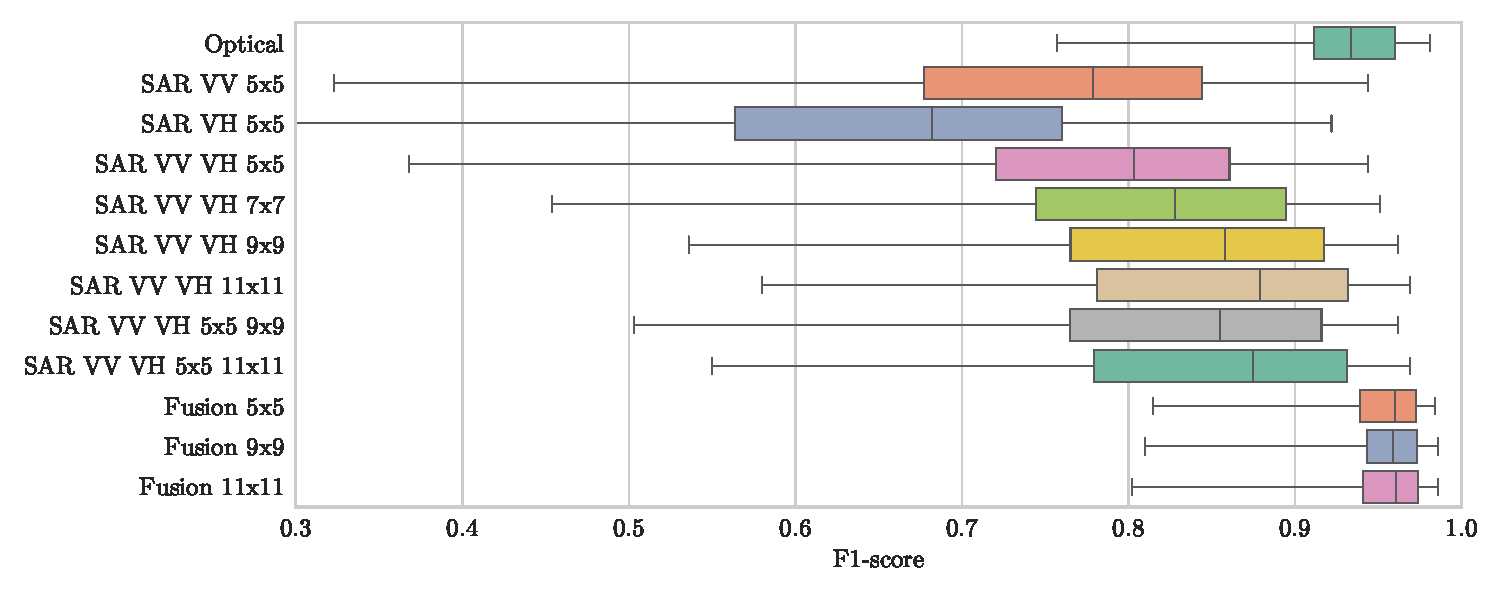
\includegraphics[width=\textwidth]{figures/score_per_scheme_boxplot.pdf}
    \caption{Box plot of the F1-score obtained with each classification
    scheme for each case study.}
    \label{fig:scores-boxplot}
\end{figure}

The performance of each classification scheme is summarised in
\autoref{fig:scores-boxplot}, which confirms the previously observed trends. The
difference between the various SAR-based classification schemes is also
highlighted. Classifications based on the VV polarization reached higher scores
compared to the ones based on the VH polarization. However, combining texture
features derived from both polarizations appears to increase the reliability of
the classification models, leading to higher scores and a lower standard
deviation. Likewise, the window size used for the computation of the GLCM did
influence the classification scores. In our case studies, larger window sizes
led to higher scores and reduced the variability across the case studies. We
previously stated the hypothesis that combining several window sizes could
increase the classification performance by including spatial information from
multiple scales. The results obtained tend to refute this hypothesis, as the
schemes combining textures from two window sizes did not perform better.
Generally, the fusion schemes consistently obtained the highest scores. However,
contrary to the trend observed in single-sensor SAR-based schemes, combining
optical data with larger window sizes textures does not seem to increase the
classification performance. Fusion schemes that include textures computed with
smaller window sizes (\(5 \times 5\) and \(9 \times 9\)) benefited from slightly
less variability across the case studies.

\begin{figure}[H]
    \centering
    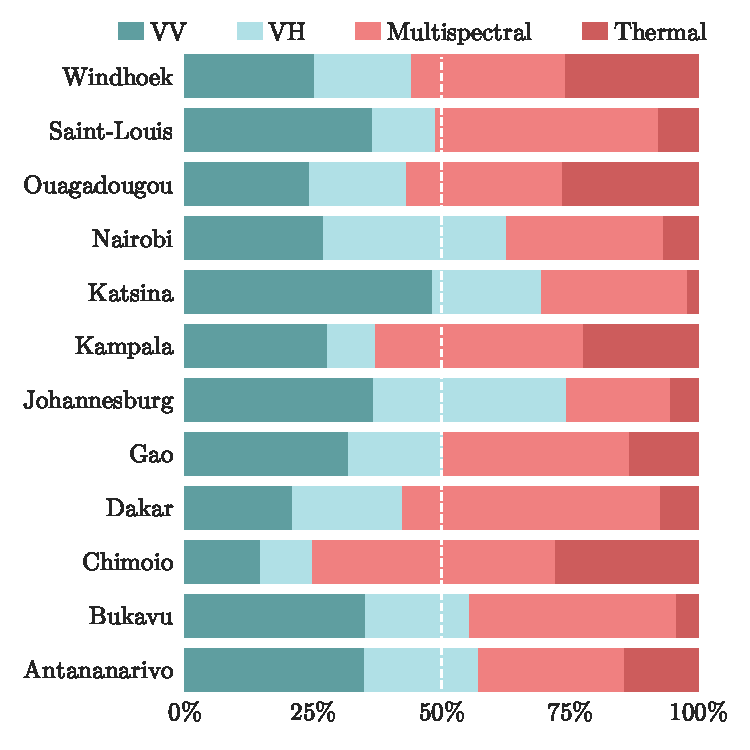
\includegraphics[width=8cm]{figures/feature_importances.pdf}
    \caption{Grouped Random Forest feature importances for the fusion scheme
    in each case study. VV and VH groups correspond to the SAR features
    derived from a given polarization. Multispectral and thermal groups
    correspond to the Landsat 8 bands.}
    \label{fig:feature-importances}
\end{figure}

In classifiers based on a forest of decision trees such as RF, the relative
contribution of each feature can be evaluated through the feature importance
measure. The value ranges from 0.0 to 1.0, where 0.0 would indicate a feature
that does not contribute to the classification, and 1.0 a feature that alone
classifies all samples. \autoref{fig:feature-importances} shows the repartition
of the importance measure across the input features used in the fusion
classification scheme, grouped by data source: VV or VH polarization for SAR
data, and multispectral or thermal for optical data. Generally, texture features
derived from the VV polarization and multispectral bands from Landsat 8 were the
features contributing the most to the construction of the decision trees.
Considering the lower scores obtained in single-sensor classification schemes
with SAR data, lower importances for SAR features could be expected. However,
the grouped importance of SAR features was superior to the importance of optical
features in 5 case studies, and exceeded 40\% of the contribution in 10 case
studies. Furthermore, the relative importance of optical and SAR features did
not appear correlated with their respective scores in the context of a
single-sensor classification. For instance, in Antananarivo and Nairobi, the
best SAR-based classification scheme reached a F1-score lower than the
optical-based scheme by, respectively, 4.2 and 3.9 points. However, in the
context of the fusion scheme, the contribution of SAR features was superior to
the contribution of optical features. This suggests that the combination of both
optical and SAR features adds information to the classifier that cannot be
modeled in the context of a single-sensor classification.

\begin{figure}[H]
    \centering
    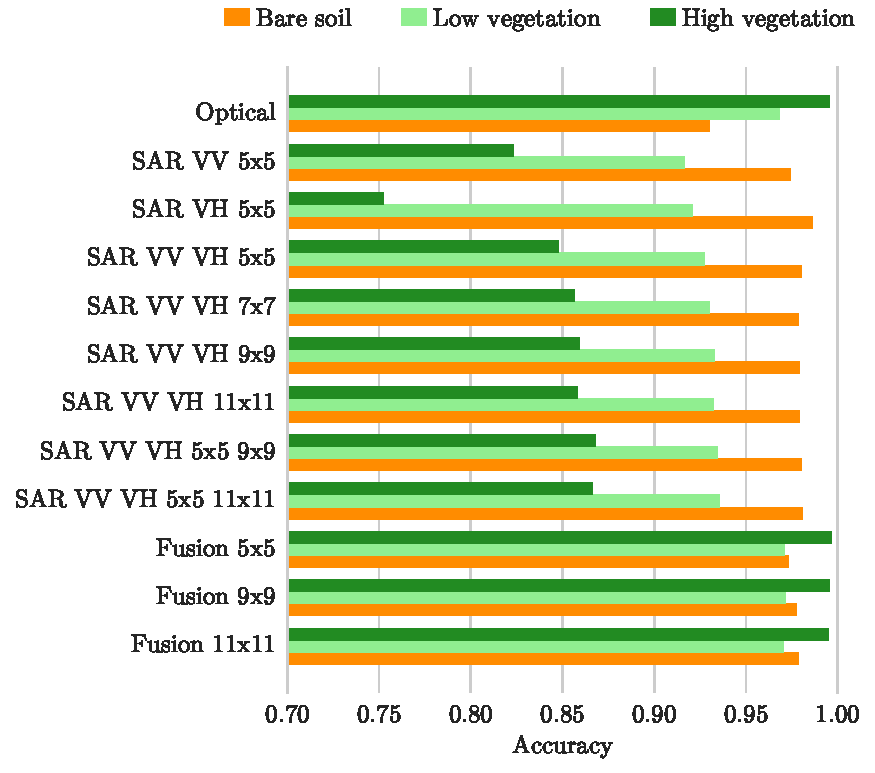
\includegraphics[width=10cm]{figures/accuracy_per_landcover.pdf}
    \caption{Classification accuracy in specific land covers for each scheme.}
    \label{fig:accuracy-landcover}
\end{figure}

As previously stated, combining SAR-based textural information and optical
imagery is expected to improve the classification performance in bare lands.
\autoref{fig:accuracy-landcover} shows the mean accuracy of each classification
scheme in three non-built-up land covers: bare soil, low vegetation and high
vegetation. As expected, the performance of the classification model in bare
soil areas was superior in SAR-based schemes than in optical-based schemes. On
the contrary, SAR-based classification schemes, especially the ones based on the
VH polarization, suffered from low accuracies in densely vegetated areas.
Finally, fusion schemes based on both SAR and optical data benefited from the
complementarity between both sensors and present high accuracies in the three
land covers.

\begin{figure}[H]
    \centering
    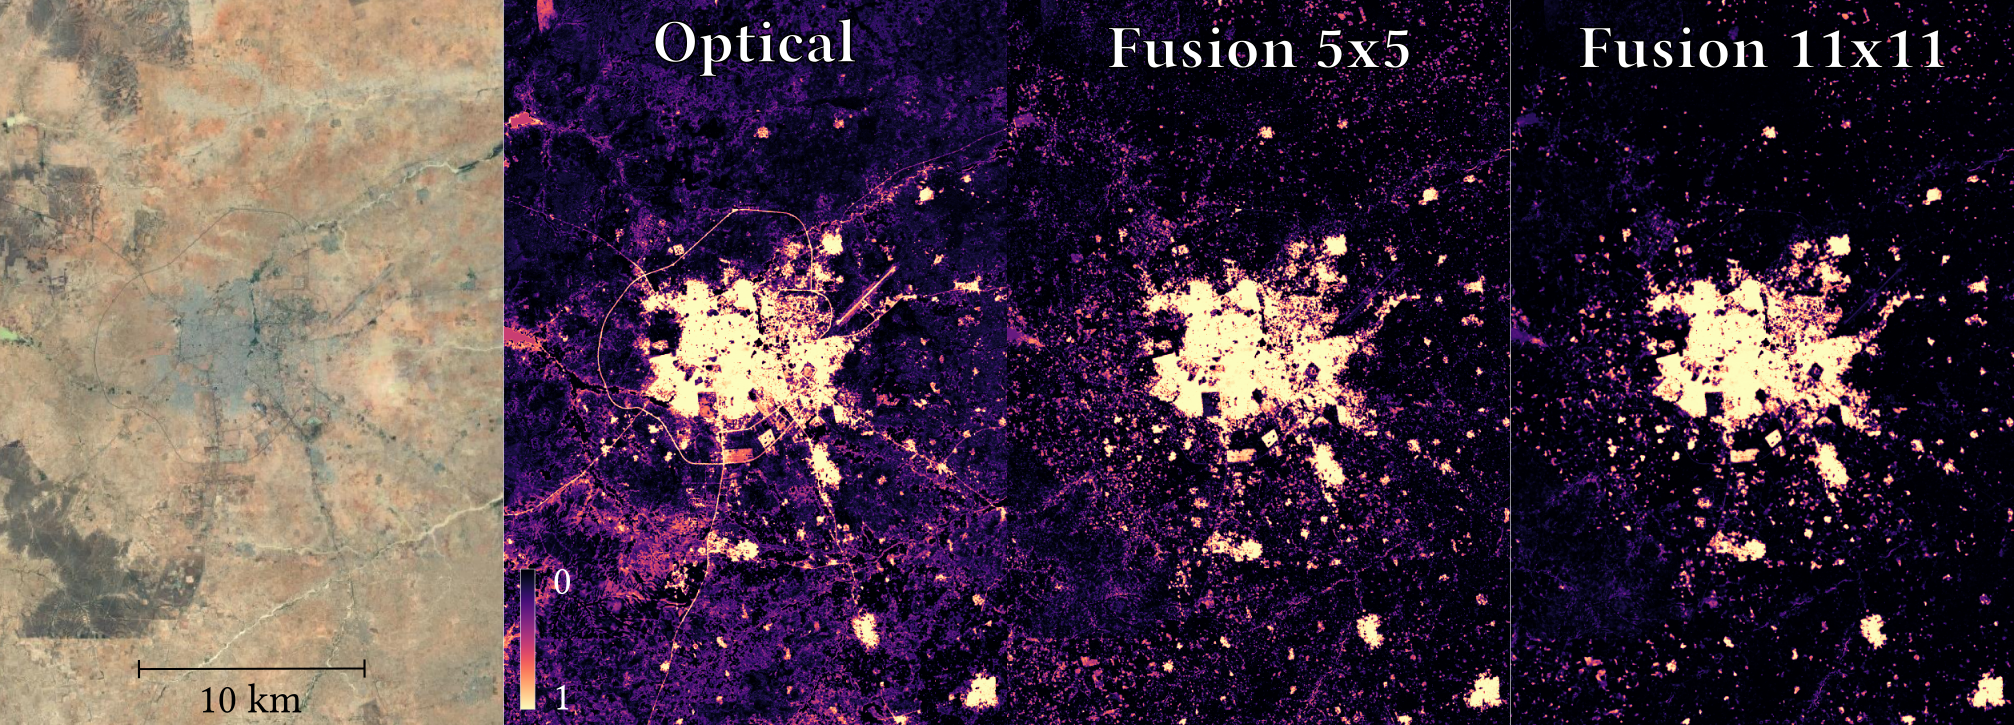
\includegraphics[width=\textwidth]{figures/katsina.png}
    \caption{Random Forest class probabilities in Katsina, Nigeria.
    \textbf{a}) Aerial view of the case study; \textbf{b}) \texttt{optical}
    scheme probabilities; \textbf{c}) \texttt{fusion\_5x5} scheme
    probabilities; \textbf{d}) \texttt{fusion\_11x11} scheme probabilities.
    Satellite imagery courtesy of Google.}
    \label{fig:katsina}
\end{figure}

\autoref{fig:katsina} shows the probabilistic output of three different
classifiers: one based only on optical data, and two based on both optical and
SAR data with different GLCM window sizes. Visually, the fusion classifiers
appears to better distinguish between the built-up areas and the surrounding
bare lands. This leads to lower rates of misclassification after thresholding of
the probabilities, as previously shown by the assessment metrics. A side effect
of the data fusion is the disappearance of the road network from the built-up
class. Indeed, the classifier highly relies on the textural information from the
SAR features to discriminate between built-up and bare land, and roads are
therefore excluded from the built-up class.

\begin{figure}[H]
    \centering
    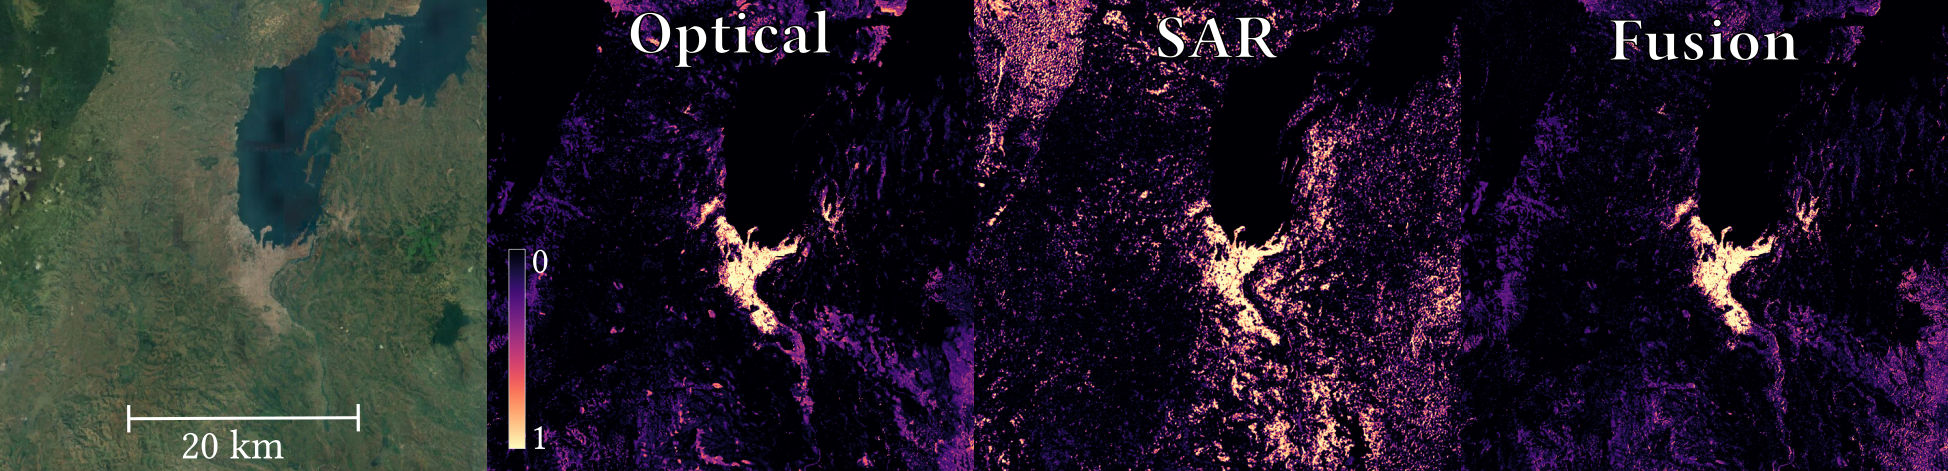
\includegraphics[width=\textwidth]{figures/bukavu.png}
    \caption{Random Forest class probabilities in Bukavu, D. R. Congo.
    \textbf{a}) Aerial view of the case study; \textbf{b}) \texttt{optical}
    scheme probabilities; \textbf{c}) \texttt{sar\_vv\_vh\_5x5\_11x11}
    scheme probabilities; \textbf{d}) \texttt{fusion\_11x11} scheme
    probabilities. Satellite imagery courtesy of Google.}
    \label{fig:bukavu}
\end{figure}

There is some cases where data fusion is less beneficial. \autoref{fig:bukavu}
shows the probabilistic output of the optical, SAR, and fusion schemes in
Bukavu. This case study, located in a mountainous area, presents two major
obstacles for SAR data: dense vegetation in the north-west and steep slopes in
the south-east. Mapping the probabilistic output of the SAR-based classifier
reveals the confusion occurring in these areas. As a result, the probabilistic
output of the fusion-based classifier appears nearly as a copy of the
optical-based one.

\section{Conclusion}

With the increasing availability of free imagery from multiple sensors such as
Sentinel-1 and Landsat 8, data fusion is one of the main challenge in remote
sensing. The objective of this paper was to assess the combined use of both
Landsat 8 and Sentinel-1 imagery with a fusion scheme that relies on a simple
pixel-based classifier. The main expectation was a better discrimination between
built-up and bare soil areas in the context of urban mapping in Sub-Saharan
Africa. The presented results suggest that the complementarity between medium
resolution optical and SAR sensors can be exploited in the context of a
supervised pixel-based classification. However, to make the pixel-based approach
effective, textural information must be extracted from SAR backscattering in
order to reduce the speckle noise and to provide contextual information at the
pixel level.

Classification schemes including both optical and SAR features reached the
highest scores in 11 case studies out of 12. Single-sensor classifiers making
use of GLCM textures derived from the VV polarization outperformed the ones
based on the VH polarization. Nevertheless, combining both polarizations
consistently increased the classification performance. Likewise, large GLCM
window sizes (\(9 \times 9\) or \(11 \times 11\)) provided a slight improvement
of the classification performance both in the context of single-sensor
classification and in fusion schemes. However, contrary to an hypothesis that we
formulated, combining textures derived from multiple GLCM window sizes --- in
order to include spatial information from multiple scales at the pixel level,
did not lead to a better classification performance. The visual interpretation
of the results obtained suggests that small GLCM window sizes favor the
detection of isolated settlements and buildings, whereas larger window sizes
lead to a better differentiation between built-up areas and bare lands. In the
context of this study, the RF classifier was not able to take advantage of both.

The assessment of the classifiers performances in specific land covers confirmed
the high level of complementarity between the two sensors. Single-sensor
SAR-based classifications presented high accuracies in bare soil areas, but
suffered from a confusion between dense vegetation and buildings. On the
contrary, optical-based classifiers showed a high ability to discriminate
between vegetation and built-up, but a low differentiation between bare soil and
built-up --- especially in the most arid landscapes such as in Gao or Katsina.
This complementarity was correctly modeled by the RF classifier and, as a
result, the fusion schemes presented high accuracies in both bare lands and
vegetated areas.

Nevertheless, the fusion was less beneficial in case studies characterized by
the presence of dense vegetation and steep slopes --- for instance in a
mountainous and subtropical urban areas such as Bukavu. However, in this case,
the RF classifier was able to learn from the training dataset that SAR data were
not reliable. This suggests that including features derived from a DEM --- for
instance slope and aspect, could improve the model ability to quantify the
reliability of SAR data at the pixel level. Such a strategy could also take
place at the decision level. Further work is also required to assess the
reliability of the presented approach in the context of similar sensors such as
Sentinel-2, ERS-1 and ERS-2.

\authorcontributions{Conceptualization, Y.F., M.S., C.L., M.G.; Data curation,
Y.F.; Formal analysis, Y.F., M.S.; Funding acquisition, C.L., M.G., M.S.;
Investigation, Y.F.; Methodology, Y.F., M.S.; Project administration, C.L., M.G.,
M.S.; Resources, M.G.; Software, Y.F.; Supervision, C.L., M.S., M.G.;
Validation, Y.F., C.L., M.S., M.G.; Visualization, Y.F.; Writing - original
draft, Y.F.; Writing - review \& editing, Y.F., M.S., M.G., C.L.}

\funding{This research was funded by the Belgian Science Policy Office and is part of the research project
SR/00/304 MAUPP (Modelling and Forecasting African Urban Population Patterns for Vulnerability and Health
Assessments).}

\conflictsofinterest{The authors declare no conflict of interest.}

\externalbibliography{yes}
\bibliography{references.bib}

\end{document}
